\chapter {Element Attributes}
\label{c:attrib}
\index{element attribute}

%-----------------------------------------------------------------
\section{Dependent and Independent Attributes} 
\label{s:depend} 
\index{element attribute!dependent and independent}

\index{parameter statement}
\index{dependent attribute}
For convenience, \bmad computes the values of some attributes based
upon the values of other attributes. These dependent variables are
listed in Table~\ref{t:dependent}. Also shown in
Table~\ref{t:dependent} are the independent variables they are
calculated from.  In the table \vn{n_part} and \vn{l_lattice} (lattice
length) are lattice attributes, not element attributes. The first two
are set by the \vn{parameter} statement (See
\sref{s:param}). \vn{l_lattice} is calculated when the
lattice is read in.

\index{bbi_constant}\index{charge}\index{sig_x}\index{sig_y}
\index{e_tot}\index{n_part}\index{e_field}\index{voltage}
\index{hkick}\index{vkick}\index{gap}\index{l}
\index{e_tot}\index{e_loss}\index{delta_e}\index{gradient}
\index{l}\index{rho}\index{angle}\index{l_chord}
\index{g}\index{l}\index{k1}\index{rho}\index{num_steps}\index{ds_step}
\index{b_max}\index{e_tot}\index{beambeam}\index{elseparator}
\index{lcavity}\index{rbend}\index{sbend}\index{wiggler}
\begin{table}[ht]
\centering {
\begin{tabular}{|l|l|l|} \hline
 {\em Element}                & {\em Independent Variables}    & {\em Dependent Variables}          \HH
 All elements                 & \vn{ds_step}                   & \vn{num_steps}                     \HH
 \vn{BeamBeam}                & \vn{charge}, \vn{sig_x}, \vn{sig_y}, \vn{e_tot}, \vn{n_part}
                                                               & \vn{bbi_constant}                  \HH
 \vn{Elseparator}             & \vn{hkick}, \vn{vkick}, \vn{gap}, \vn{l}, \vn{e_tot}      
                                                               & \vn{e_field}, \vn{voltage}         \HH
 \vn{Lcavity}                 & \vn{gradient}, \vn{l}          & \vn{e_loss}, \vn{delta_e}          \HH
 \vn{Rbend}, \vn{Sbend}       & \vn{g}, \vn{l}                     
                                                               & \vn{rho}, \vn{angle}, \vn{l_chord} \HH

 \vn{Wiggler} (map type)      & \vn{term(i)}                   & \vn{b_max}, \vn{k1}, \vn{rho}      \HH
 \vn{Wiggler} (periodic type) & \vn{b_max}, \vn{e_tot}         & \vn{k1}, \vn{rho}                  \HH
\end{tabular}
}
\caption[Table of dependent variables.]{Table of dependent variables and 
  the independent variables 
they are calculated from.}
\label{t:dependent}
\end{table}

\index{lattice!expansion}\index{harmon}\index{delta_e}\index{gradient}
\index{rho}\index{g}\index{angle}\index{rf_frequency}
No attempt should be made to set or vary within a program dependent
attributes. It should be remarked that this is not an iron clad rule.
If a program properly bypasses \bmad's attribute bookkeeping routine
then anything is possible. In a lattice file, before lattice expansion
(\sref{s:expand}), \bmad allows the setting of a select group of
dependent attributes if the appropriate independent attributes are
not set. The list of settable dependent variables is given in
Table~\ref{t:dep.except}.  After reading in the lattice \bmad will set
the appropriate independent variable based upon the value of the
dependent variable. \vn{harmon} is the exception in that it will never
be set by the bookkeeping routine.
\index{lcavity}\index{rbend}
\index{sbend}\index{rfcavity}
\begin{table}[ht]
\centering {
\begin{tabular}{|l|l|l|} \hline
{\em Element}                  & {\em Dependent Variable Set}  &  {\em Independent Variables Not Set} \HH
  \vn{Lcavity}                 & \vn{delta_e}       & \vn{gradient}      \HH
  \vn{Rbend}, \vn{Sbend}       & \vn{rho}           & \vn{g}             \HH
  \vn{Rbend}, \vn{Sbend}       & \vn{angle}         & \vn{g}, or \vn{l}  \HH
  \vn{RFcavity}                & \vn{rf_frequency}  & \vn{harmon}        \HH
  \vn{Wiggler} (periodic type) & \vn{n_pole}        & \vn{l_pole}        \HH
\end{tabular}
}
\caption {Dependent variables that can be set in a primary lattice file.}
\label{t:dep.except}
\end{table}

\index{g}\index{g_err}\index{b_field}\index{bs_field}\index{b_field_err}
\index{b1_gradient}\index{b2_gradient}\index{b3_gradient}\index{ks}
\index{k1}\index{k2}\index{k3}
\index{bl_kick}\index{bl_hkick}\index{bl_vkick}
\index{kick}\index{hkick}\index{vkick}
The normal attribute used to vary the strength of, say, a
\vn{quadrupole} is \vn{k1}.  It is sometimes convenient to be able to
vary the magnetic field strength directly instead. To do this \bmad
has a rule that if the appropriate field attribute appears in the
primary lattice file then it becomes an independent variable and the
normalized strength attribute (the strength attribute normalized by
the reference energy) becomes a dependent variable as tabulated in
Table~\ref{t:dep.field}.
\index{sbend}\index{rbend}\index{solenoid}\index{quadrupole}
\index{sol_quad}\index{sextupole}\index{octupole}
\begin{table}[ht]
\centering {
\begin{tabular}{|l|l|l|} \hline
  {\em Element} & {\em Normalized Strength} & {\em Field Attribute} \HH
  \vn{Sbend}, \vn{Rbend}     & \vn{g}      &  \vn{b_field}        \HH
  \vn{Sbend}, \vn{Rbend}     & \vn{g_err}  &  \vn{b_field_err}    \HH
  \vn{Solenoid, Sol_quad}    & \vn{ks}     &  \vn{bs_field}       \HH
  \vn{Quadrupole, Sol_quad, Sbend, Rbend}            
                             & \vn{k1}     &  \vn{b1_gradient}    \HH
  \vn{Sextupole, Sbend, Rbend}             
                             & \vn{k2}     &  \vn{b2_gradient}    \HH
  \vn{Octupole}              & \vn{k3}     &  \vn{b3_gradient}    \HH
  \vn{HKicker}, \vn{VKicker} & \vn{kick}   &  \vn{bl_kick}        \HH
  Most                       & \vn{hkick}  &  \vn{bl_hkick}       \HH
  Most                       & \vn{vkick}  &  \vn{bl_vkick}       \HH
\end{tabular}
}
\caption {Field and Strength Attributes.}
\label{t:dep.field}
\end{table}
Using both field strength and normalized strength as the independent
variable for a given element is not permitted. For example, for a quadrupole the 
normalized strengths \vn{k1}, \vn{hkick}, and \vn{vkick} can be used as the
independent variable or the field strengths \vn{b1_gradient}, \vn{bl_hkick} and
\vn{bl_vkick}. but the mixing of the two is not valid
\begin{example}
  Q1: quadrupole, k1 = 0.6, bl_hkick = 37.5  ! NO. Not VALID.
\end{example}
\index{field_master}
To define an element with the field strength as the independent
attribute without setting the strength just set the strength to zero
or, alternatively, the \vn{field_master} logical can be set. For
example
\begin{example}
  Q1: quadrupole, b1_gradient = 0   ! Field strengths now the independent variables
  Q1: quadrupole, field_master = T  ! Same as above
\end{example}
The same effect can be obtained by setting the field or \vn{field_master} attributes
after the element has been defined.
\begin{example}
  q1: quadrupole        ! Define q1.
  q1[b1_gradient] = 0   ! Field strengths now the independent variables.
  q1[field_master] = T  ! Same as above.
\end{example}

%-----------------------------------------------------------------
\section{Type, Alias and Descrip Attributes}
\label{s:string}
\index{type|hyperbf}
\index{alias|hyperbf}
\index{descrip|hyperbf}

There are three string labels associated with any element:
\begin{example}
  type    = <String>
  alias   = <String>
  descrip = <String>
\end{example}
\bmad routines do not use these labels except when printing element
information. \vn{type} and \vn{alias} can be up to 16 characters in
length and \vn{descrip} can be up to 200 characters. The attribute
strings can be enclosed in double quotation marks ("). The attribute
strings may contain blanks. If the attribute string does not contain a
blank then the quotation marks may be omitted. In this case the first
comma (,) or the end of the line marks the end of the string. Example:
\begin{example}
  Q00W: Quad, type = "My Type", alias = Who_knows, &
                                  descrip = "Only the shadow knows"
\end{example}

%-----------------------------------------------------------------
\section[Energy and Wavelength Attributes]{Energy and Wavelength Attributes: E_tot, P0C, and ref_wavelength }
\label{s:energy}
\index{parameter statement}\index{e_tot}
\index{e_tot_start}\index{p0c_start}
\index{patch}\index{lcavity}\index{p0c}
\index{n_ref_pass}\index{ref_wave_length}
The attributes that define the reference energy and momentum at an element are:
\begin{example}
  e_tot  = <Real>  ! Total energy in eV.
  p0c    = <Real>  ! Momentum in eV.
\end{example}
The energy and momentum are defined at the exit end of the element.
For ultra--relativistic particles, and for photons, these two values
are the same (\sref{s:phase.space}). Except for multipass elements
(\sref{s:multipass}), \vn{e_tot} and \vn{p0c} are dependent attributes
and, except for multipass elements, any setting of \vn{e_tot} and
\vn{p0c} in the lattice input file is an error. The value of
\vn{e_tot} and \vn{p0c} for an element is calculated by \bmad to be
the same as the previous element except for \vn{Lcavity} and
\vn{patch} elements. To set the \vn{e_tot} or \vn{p0c} at the start of
the lattice use the \vn{beginning} or \vn{parameter} statements.
See~\sref{s:param}. Since the energy changes from the start to the end
of an \vn{Lcavity}, an \vn{Lcavity} has the dependent attributes
\begin{example}
  e_tot_start   and
  p0c_start
\end{example}
which are just the reference energy and momentum at the start of the element.

For \vn{multipass} elements, the reference energy is set by specifying
one of \vn{e_tot}, \vn{p0c}, or \vn{n_ref_pass} as described in
\sref{s:multipass}.

For photons, the reference wavelength, \vn{ref_wavelength} is also a
dependent attribute calculated from the reference energy.

%-----------------------------------------------------------------
\section{Offset, Pitch, Tilt, and Roll Attributes}
\label{s:offset}
\index{x_offset|hyperbf}
\index{y_offset|hyperbf}
\index{s_offset|hyperbf}
\index{x_pitch|hyperbf}
\index{y_pitch|hyperbf}
\index{roll|hyperbf}
\index{tilt|hyperbf}

There are up to 7 attributes that can offset a physical element
from the reference orbit. They are
\begin{example}
  x_offset = <Real>
  y_offset = <Real>
  s_offset = <Real>
  x_pitch  = <Real>
  y_pitch  = <Real>
  tilt     = <Real>
  roll     = <Real>
\end{example}
\index{patch}
The exception here is the \vn{patch} element which uses these
attributes to modify the reference orbit itself.

\vn{x_offset} translates an element in the local $x$--direction
as shown in Figure~\ref{f:pitch}. Similarly, \vn{y_offset} and 
\vn{s_offset} translate an element along the local $y$ and 
$z$--directions respectively. For a bend it is assumed that
the bend angle is small and the rotation of the local reference
axes through the bend is ignored.

The \vn{x_pitch} attribute rotates an element about the $y$--axis so
that the exit face of the element is displaced in the $+x$--direction
as shown in figure~\ref{f:pitch}. Similarly the \vn{y_pitch} attribute
rotates an element about the $x$--axis so that the exit face of the
element is displaced in the $+y$--direction. The rotations are about
the center of the element which is in contrast to the \vn{dtheta} and
\vn{dphi} misalignments of \mad which rotate around the entrance
point. In terms of rotation angle
\index{MAD!element rotation origin}
\begin{example}
  x_pitch =  dtheta
  y_pitch = -dphi
\end{example}
Since \bmad uses the small angle approximation, the pitches are
considered small so that the \vn{x_pitch} and \vn{y_pitch}
transformations commute.

\begin{figure}[t]
  \centering
  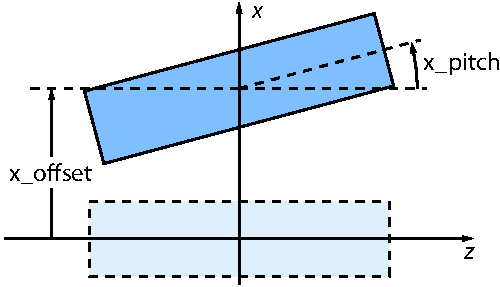
\includegraphics{pitch.pdf}
  \caption{Geometry of Pitch and Offset attributes}
  \label{f:pitch}
\end{figure}

\begin{figure}[t]
  \centering
  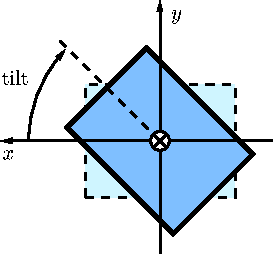
\includegraphics{tilt.pdf}
  \caption{Geometry of a Tilt}
  \label{f:tilt}
\end{figure}

The tilt attribute rotates the element in the $(x, y)$ plane as shown
in figure~\ref{f:tilt}. The rotation axis is the $z$-axis at the
entrance face. The reference orbit is also rotated for any element
who's exit coordinates are not collinear with the entrance
coordinates. For example, a \vn{bend} or \vn{mirror} with a tilt of
$\pi/2$ will bend a beam vertically upward. The \vn{hkick} and
\vn{vkick} attributes are not affected by \vn{tilt} except for
\vn{Kicker} and \vn{ElSeparator} elements. Like MAD, \bmad allows the
use of the \vn{tilt} attribute without a value to designate a skew
element. For example
\begin{example}
  q1: quad, l = 0.6, x_offset = 0.03, y_pitch = 0.001, tilt
\end{example}
\index{rbend!tilt default}\index{sbend!tilt default}
\index{sol_quad!tilt default}\index{quadrupole!tilt default}
\index{sextupole!tilt default}\vn{octupole!tilt default}
Default tilts can be used for \vn{rbend}, \vn{sbend}, \vn{sol_quad},
\vn{quadrupole}, \vn{sextupole}, and \vn{octupole} elements.
The default tilt is $\pi/(2(n+1))$ where $n$ is the order of the 
element (n = 0 for bends, n = 1 for quadrupoles etc.) 

\index{sbend}\index{rbend}\index{crystal}\index{mirror}
For all elements, except \vn{crystal} and \vn{mirror} elements,
offsets and pitches and are measured with respect to the local coordinates at the
center of the element. \vn{Crystal} and \vn{mirror} elements measure
their offsets and pitches with respect to the entrance coordinates.
Note that all element define \vn{tilt} with respect to the entrance
coordinates.

The \vn{roll} attribute is only used for bends and rotates the bend,
along an axis that runs through the entrance point and exit point as
shown in figure~\ref{f:roll}. A \vn{roll}, unlike a \vn{tilt}, does not affect the
reference orbit. The major effect of a \vn{roll} is to give a vertical
kick to the beam. For a bend with positive bend angle, a positive
\vn{roll} will move the outside portion ($+x$ side) of the bend upward
and the inside portion (-$x$ side) downward. Much like car racetracks
which are typically slanted towards the inside of a turn.

\begin{figure}[ht]
  \centering
  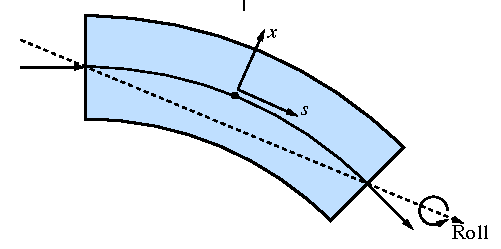
\includegraphics{roll.pdf}
  \caption[Geometry of a Bend]{
Geometry of a Bend. A roll is a rotation around the axis passing
through the entrance and exit points. Like most other elements,
offsets and pitches are calculated with respect to the coordinates at
the center of the bend. Shown here is the geometry for a bend with
\vn{tilt} = 0. That is, the bend is in the $x-s$ plane.}
  \label{f:roll}
\end{figure}

\index{x_offset_tot|hyperbf}\index{y_offset_tot|hyperbf}\index{s_offset_tot|hyperbf}
\index{x_pitch_tot|hyperbf}\index{y_pitch_tot|hyperbf}
\index{tilt_tot|hyperbf}
If an element is supported by a \vn{girder} element (\sref{s:girder}),
the offsets, pitches and tilt of the element are with respect to the
orientation of the \vn{girder}. The computed offsets, pitches and tilt with
respect to the local reference coordinates are stored in the dependent attributes
\begin{example}
  x_offset_tot
  y_offset_tot
  s_offset_tot
  x_pitch_tot
  y_pitch_tot
  tilt_tot
\end{example}
If an element is not supported by a \vn{girder}, \vn{x_offset_tot}
will have the same value as \vn{x_offset} etc.

%-----------------------------------------------------------------
\section{Hkick, Vkick, and Kick Attributes}
\label{s:kick}
\index{hkick|hyperbf}\index{bl_hkick|hyperbf}
\index{vkick|hyperbf}\index{bl_vkick|hyperbf}
\index{kick|hyperbf}\index{bl_kick|hyperbf}


\index{hkicker}
\index{vkicker}
\index{elseparator}
\index{kicker}
The kick attributes that an element may have are:
\begin{example}
  kick,  bl_kick  = <Real>  ! Used only with a Hkicker or Vkicker
  hkick, bl_hkick = <Real>
  vkick, bl_vkick = <Real>
\end{example}
\vn{kick}, \vn{hkick}, and \vn{vkick} attributes are the integrated
kick of an element in radians. \vn{kick} is only used for \vn{Hkicker}
and \vn{Vkicker} elements. All other elements that can kick use
\vn{hkick} and \vn{vkick}. The \vn{tilt} attribute will only rotate a
kick for \vn{Hkicker}, \vn{Vkicker}, \vn{Elseparator} and \vn{Kicker}
elements. This rule was implemented so that, for example, the
\vn{hkick} attribute for a skew quadrupole would represent a
horizontal steering. The \vn{bl_kick}, \vn{bl_hkick}, and
\vn{bl_vkick} attributes are the integrated field kick in
\vn{meters-Tesla}. Normally these are dependent attributes except if
they appear in the lattice file (\sref{s:depend}).

%-----------------------------------------------------------------
\section{Aperture and Limit Attributes}
\label{s:limit}
\index{aperture|hyperbf}
\index{limit|hyperbf}
\index{aperture_at|hyperbf}

\begin{figure}[ht]
  \centering
  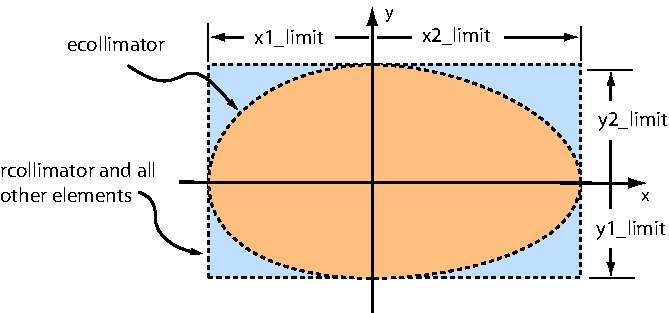
\includegraphics{apertures.pdf}
  \caption[Apertures for ecollimator and rcollimator elements.]
  {Apertures for ecollimator and rcollimator elements. 
  Positive $s$ points up out of the page.}
  \label{f:limit}
\end{figure}

\index{ecollimator}
\index{rcollimator}
\index{x_limit|hyperbf}
\index{y_limit|hyperbf}
\index{x1_limit|hyperbf}
\index{y1_limit|hyperbf}
\index{x2_limit|hyperbf}
\index{y2_limit|hyperbf}
\index{x_offset|hyperbf}
\index{offset_moves_aperture|hyperbf}
\index{aperture_type}
The aperture attributes are:
\begin{example}
  x1_limit      = <Real>      ! Horizontal, negative side, aperture limit
  x2_limit      = <Real>      ! Horizontal, positive side, aperture limit
  y1_limit      = <Real>      ! Vertical, negative side, aperture limit
  y2_limit      = <Real>      ! Vertical, positive side, aperture limit
  x_limit       = <Real>      ! Alternative to specifying x1_limit and x2_limit
  y_limit       = <Real>      ! Alternative to specifying y1_limit and y2_limit
  aperture      = <Real>      ! Alternative to specifying x_limit and y_limit
  aperture_at   = <Switch>    ! What end aperture is at.
  aperture_type = <Switch>    ! What type of aperture it is.
  offset_moves_aperture = <Logical> ! Element offsets affect aperture position
\end{example}
\vn{x1_limit}, \vn{x2_limit}, \vn{y1_limit}, and \vn{y2_limit} specify
the half--width of the aperture of an element as shown in
figure~\ref{f:limit}. A zero \vn{x1_limit}, \vn{x2_limit},
\vn{y1_limit}, or \vn{y2_limit} is interpreted as no aperture in the
appropriate plane.

By default, apertures are assumed to be
rectangular except that an \vn{Ecollimator} has a elliptical aperture.
This can be changed by setting the \vn{aperture_type} attribute. The possible 
values of this attribute are:
\begin{example}
  rectangular
  elliptical
\end{example}

To avoid numerical overflow and other errors in tracking, a particle
will be considered to have hit an aperture in an element, even if
there are no apertures set for that element, if its orbit exceeds 1000
meters. Additionally, there are other situations where a particle will
be considered lost. For example, if a particle's trajectory does
not intersect the output face in a bend.

For convenience, \vn{x_limit} can be used to set \vn{x1_limit} and
\vn{x2_limit} to a common value. Similarly, \vn{y_limit} can be used
to set \vn{y1_limit} and \vn{y2_limit}.  The \vn{aperture} attribute
can be use to set all four \vn{x1_limit}, \vn{x2_limit}, \vn{y1_limit}
and \vn{y2_limit} to a common value. Internally, the \bmad code does {\em not}
store \vn{x_limit}, \vn{y_limit}, or \vn{aperture}. This means that
using \vn{x_limit}, \vn{y_limit} or aperture in arithmetic expressions is
an error:
\begin{example}
  q2: quad, aperture = q1[aperture]   ! THIS IS AN ERROR!
  q2: quad, aperture = q1[x1_limit]   ! Correct
\end{example}

\index{tilt}
\index{x_offset}
\index{y_offset}
\index{x_pitch}
\index{y_pitch}
Normally, whether a particle hits an aperture or not is evaluated
independent of any element offsets (\sref{s:offset}). This is
equivalent to the situation where a beam pipe containing an aperture
is independent of the element the beam pipe passes through. This can
be changed by setting the \vn{offset_moves_aperture} attribute to
\vn{True}. In this case any offsets or pitches will be considered to
have shifted the aperture boundary. The exception here is that the
default for \vn{rcollimator} and \vn{ecollimator} elements is for
\vn{offset_moves_aperture} to be \vn{True}.

Even with \vn{offset_moves_aperture} set to \vn{True}, \vn{tilt}s will
not affect the aperture calculation. This is done, for example, so
that the tilt of a skew quadrupole does not affect the aperture. The
exception here is that tilting an \vn{rcollimator} or \vn{ecollimator}
element will tilt the aperture.

\index{entrance_end|hyperbf}
\index{exit_end|hyperbf}
\index{aperture_at}
By default the aperture is evaluated at the exit face only of the
element. This can be changed by setting the \vn{aperture_at} attribute.
Possible settings for \vn{aperture_at} are:
\begin{example}
  entrance_end
  exit_end  ! default
  both_ends
\end{example}
Note that the entrance and exit ends of an element are independent of
which direction particles are tracked through an element. Thus if a
particle is tracked backwards it enters an element at the ``exit end''
and exits at the ``entrance end''.

Examples:
\begin{example}
  q2: quad, aperture_type = elliptical  
  q1: quad, l = 0.6, x1_limit = 0.045, offset_moves_aperture = T
  q1[y1_limit] = 0.03
  q1[y2_limit] = 0.03
  q1[y_limit] = 0.03  ! equivalent to the proceeding 2 lines.  
  q1[aperture_at] = both_ends
\end{example}

%-----------------------------------------------------------------
\section{Length Attributes}
\label{s:l}

\index{length of elements}
\index{l|hyperbf}
\index{l_chord|hyperbf}
\index{rbend}
\index{sbend}
The length attributes are
\begin{example}
  l       = <Real>  ! 
  l_chord = <Real>  ! Chord length of a bend. Dependent attribute.
\end{example}
The length \vn{l} is the path length of the reference particle. The
one exception is for an \vn{Rbend}, the length \vn{l} set in the
lattice file is the chord length (\sref{s:bend}). Internally, \bmad
converts all \vn{Rbend}s to \vn{Sbend}s and stores the chord length
under the \vn{l_chord} attribute.

\index{wiggler}
Note that for \vn{Wiggler}s,
the length \vn{l} is not the same as the path length for a particle
with the reference energy starting on the reference orbit.

%-----------------------------------------------------------------
\section{Is_on Attribute}
\label{s:is.on}
\index{is_on|hyperbf}

The \vn{is_on} attribute
\begin{example}
  is_on = <Logical>
\end{example}
is used to turn an element off. Turning
an element off essentially converts it into a drift.
Example
\begin{example}
  q1: quad, l = 0.6, k1 = 0.95
  q1[is_on] = False
\end{example}

\index{aperture}
\index{reference orbit}
\index{reference energy}
\vn{is_on} does not affect any apertures that are set. Additionally,
\vn{is_on} does not affect the reference orbit. Therefore, turning 
off an \vn{lcavity} will not affect the reference energy.

%-----------------------------------------------------------------
\section{Multipole Attributes: An, Bn, KnL, Tn}
\label{s:multip}

\index{multipole!an, bn|hyperbf} 
\index{multipole!knl, tn|hyperbf} 
\index{ab_multipole}
\index{multipole}
\index{radius}
A \vn{multipole} (\sref{s:mult}) element specifies its multipole
components using an Amplitude (\vn{KnL}) and a tilt (\vn{Tn})
\begin{example}
  KnL = <Real>
  Tn  = <Real>  ! Default is $pi$/(2n + 2)
\end{example}
\vn{AB_Multipole} (\sref{s:ab.m}) and all other elements that
have multipole attributes specify the multipoles using normal
(\vn{Bn}) and skew (\vn{An}) components 
\begin{example}
  An = <Real>
  Bn = <Real>
\end{example}
Here \vn{n} ranges from 0
(dipole component) through 20. Example:
\begin{example}
  q1: ab_multipole, b0 = 0.12, a20 = 1e7
\end{example}

Multipole formulas for are given in \sref{s:fields}.  Note that for
\vn{Multipole} and \vn{AB_multipole} (but not any other element) a
non-zero dipole component will affect the reference orbit (just like a
normal dipole will).

The \vn{Tn} tilt component without a value takes a default of $pi$/(2n + 2) which makes
the component \vn{skew}.
Example:
\begin{example}
  m: multipole, k1l = 0.45, t1  ! Skew quadrupole
\end{example}

For everything other than a \vn{Multipole} and \vn{AB_multipole}, the
multipole strength is scaled by a factor $F \, r_0^{n_\text{ref}} /
r_0^n$ (cf.~\Eq{ababf}) where $F$ is the strength of the element (for
example $F$ is $K1 \cdot L$ for a quadrupole), and $r_0$ is the
``measurement radius'' and is set by the \vn{radius} attribute. The
default value of $r_0$, if the \vn{radius} is not given, is 1.0.
This behavior may be turned off by setting the \vn{scale_multipoles} attribute.
Example:
\begin{example}
  q1: quadrupole, b0 = 0.12, a20 = 1e7, scale_multipoles = F
\end{example}

%-----------------------------------------------------------------
\section{RF Couplers}
\label{s:rf.coupler}

\index{coupler_at}\index{coupler_strength}
\index{coupler_angle}\index{coupler_phase}
For \vn{lcavity} and \vn{rfcavity} elements, the attributes that
characterize the dipole transverse kick due to a coupler port are:
\begin{example}
  coupler_at       = <Switch> ! What end the coupler is at
  coupler_strength = <Real>   ! Normalized strength
  coupler_angle    = <Real>   ! Polarization angle (rad/2\(\pi\))
  coupler_phase    = <Real>   ! Phase angle with respect to the RF (rad/2\(\pi\))
\end{example}
The possible \vn{coupler_at} settings are:
\begin{example}
  entrance_end
  exit_end  ! default
  both_ends
\end{example}
For \vn{coupler_angle} = 0 the transverse kick due to the coupler is
\begin{example}
  dp_x = gradient * coupler_strength * 
                        cos(twopi * (phi_ref + coupler_phase + phi(z))) / (c * P_0) 
  dp_y = 0
\end{example}

Example:
\begin{example}
  rf1: lcav, l = 4.5, gradient = 1.2e6, coupler_at = both_ends, coupler_strength = 0.037
\end{example}

%-----------------------------------------------------------------
\section{RF Wakes}
\label{s:rf.wakes}

Wake fields can be specified for \vn{lcavity} and \vn{rfcavity} elements.
The attributes that characterize the wakes are:
\index{sr_wake_file}\index{lr_wake_file}\index{lr_freq_spread}
\begin{example}
  sr_wake_file     = <String> ! Short range wake field definition file.
  lr_wake_file     = <String> ! Long range wake field definition file.
  lr_freq_spread   = <Real>   ! Frequency spread of the LR wake fields.
\end{example}

The formulas used to compute the wake field are given in
\sref{s:wake.fields}.  The input file name for the short--range
wake fields is specified using the \vn{sr_wake_file} attribute. The
file gives both monopole longitudinal and dipole transverse
wakes. Comment lines may be included by starting a line with an
exclamation mark (!). Blank lines are also ignored.  An example input
file is:
\begin{example}
  !    z           Wz             Wt
  !   [m]       [V/C/m]       [V/C/m^2]
   0.000E+00  1.61125E+15   0.00000E+00     1 
  -1.000E-05  1.44516E+15  -1.30560E+15     2 
  -2.000E-05  1.38148E+15  -2.50665E+15     3 
  .. etc ..
  -1.970E-03  3.49958E+14  -7.95507E+16   198 
  -1.980E-03  3.48606E+14  -7.97253E+16   199  
  -1.990E-03  3.47263E+14  -7.98989E+16   200
     END_SECTION


  ! Pseudo Wake modes:
  !                      Amp       damp          k      phase
  ! Longitudinal:      [V/C/m]     [1/m]      [1/m]     [rad]  
  ! Transverse:      [V/C/m^2]     [1/m]      [1/m]     [rad]  

  &short_range_modes
    longitudinal(1) = 3.23e14     1.23e3     3.62e3     0.123
    longitudinal(2) = 6.95e13     5.02e2     1.90e3    -1.503
    .. etc ..
    transverse(1) =   4.23e14     2.23e3     5.62e3     0.789
    transverse(2) =   8.40e13     5.94e2     1.92e3     1.455
     .. etc ..
    z_max = -1.3e-3
  /
\end{example}
The file is divided into two sections with a line containing the word
\vn{END_SECTION} marking the division between the sections.  Wakes can
be specified via a table of wake versus longitudinal position $z$
and/or using a set of ``pseudo'' modes (\sref{s:wake.fields}). The
first section gives the wake vs $z$ table, and the second section
gives the longitudinal monopole and transverse dipole pseudo modes.
The range of the table is from $0$ to $z_{cut}$ where $z_{cut}$ is the
$z$ value in the last line of the table. If the longitudinal distance
$dz$ between two particles is within the range of the table then the
table will be used to calculate the wake kick for this pair. If $dz$
is larger than $z_{cut}$ the pseudo modes will be used. The pseudo
modes are valid from $z_{cut}$ to \vn{z_max}. 

In the first section with the table of wake vs. $z$, the first column is the
longitudinal distance $z$. $z$ must start at 0 and must increment by the a
constant amount from row to row. $z$ is negative since the wake extends behind
a particle. The second column is the longitudinal wake function in $V/C/m$. The
third column is the transverse wake in $V/C/m^2$. Any additional columns are
ignored.  Wake field formulas are to be found in \sref{s:wake.fields}.  The
wake field file is only used with macroparticle and particle distribution
tracking.  When the short--range wake field file is used with either of these
the \vn{e_loss} attribute is ignored. However, even in this case, a finite
\vn{e_loss} value will affect the reference energy. Since the quantities like
quadrupole k1 strengths and bend strengths are referenced to the reference
energy, The value of \vn{e_loss} will affect the results even with a
short--range wake field file.

The input file name for the long--range wake fields is specified using
the \vn{lr_wake_file} attribute. The file gives the
wake modes by specifying the frequency (in Hz), R/Q (in
$\Omega$/meter$^{2m}$), Q, and m (order number), and optionally the
polarization angle (in radians/2pi) for each cavity mode. The input
uses Fortran90 namelist syntax: The data begins with the string
\vn{\&long_range_modes} and ends with a \vn{/}. Everything outside is
ignored. Each mode is labeled \vn{lr(i)} where \vn{i} is the mode
index. An example input file is:
\begin{example}
              Freq      R/Q      Q    m   Polar   b_sin  b_cos a_sin  a_cos  t_ref 
                      [Ohm/               Angle 
              [Hz]     m^(2m)]           [Rad/2pi]
  &long_range_modes
    lr(1) = 1.650e9    0.76    7.0e4  1    unpol
    lr(2) = 1.699e9   11.21    5.0e4  1    0.15
  /
\end{example}
If ``\vn{unpolarized}'' is used for the polarization angle, the mode
is taken to be unpolarized.

\vn{lr_freq_spread} is used to randomly spread out the long range mode
frequencies among different cavities. The spread is Gaussian in shape
with an RMS of \vn{lr_freq_spread} * $F$ where $F$ is the frequency of a
mode.  After the long--range modes have been defined they can be
referenced or redefined using the notation
\begin{example}
  lr(n)%freq      ! Frequency
  lr(n)%r_over_q  ! R/Q
  lr(n)%q         ! Q
  lr(n)%angle     ! Polarization Angle
\end{example}
Example:
\begin{example}
  lcav[lr(2)%freq] = 1.1 * lcav[lr(2)%freq] ! Raise frequency by 10\%
\end{example}

Example:
\begin{example}
  rf1: lcav, l = 4.5, gradient = 1.2e6, sr_wake_file = "sr1.dat"
\end{example}

%-----------------------------------------------------------------
\section{RF Fields}
\label{s:rf.fields}

For \vn{lcavity} and \vn{rfcavity} elements, the RF field can be
parameterized as the sum over a number of modes. With such a
characterization, particles can be tracked through a cavity using
\vn{boris}, \vn{adaptive_boris}, \vn{runge_kutta}, or
\vn{symp_lie_bmad} tracking (\sref{s:tkm}).

The basic equations used for the mode decomposition of the rf fields
are given in Section~\sref{s:rf.fields.phys}. The syntax for specifying the 
RF fields is
\begin{example}
  rf_field = {
    mode = {
      m             = <Integer>,
      freq          = <Real>,  ! frequency of oscillations.
      theta_t0      = <Real>,  ! Phase of oscillations. Default = 0.
      f_damp        = <Real>,  ! Oscillation damping factor. Default = 0.
      stored_energy = <Real>,  ! Default = 0.
      dz            = <Real>,  ! Distance between sampled field points.
      sample_radius = <Real>,  ! Default = 0.
      phi_0         = <Real>,  ! Azimuthal orientation.
      e_re = (<Real>, <Real>, ....),  ! Real part of e.
      e_im = (<Real>, <Real>, ....),  ! Imaginary part of e.
      b_re = (<Real>, <Real>, ....),  ! Real part of b.
      b_im = (<Real>, <Real>, ....)}, ! Imaginary part of b.
    mode = {...}}
\end{example}
The \vn{sample_radius} of a mode gives the radius $R$ where the field
data was calculated (cf.~\Eq{erpze}). This quantity is not needed for
tracking and is not used by any \bmad routines.

\vn{e_re} and \vn{e_im} give the real an imaginary part of $e$ and
\vn{b_re} and \vn{b_im} give the real and imaginary part of $b$. All
of these vectors must be present and have the same length. The
exception is with an $m = 0$ mode either the $e$ or $b$ arrays can be
omitted and will default to zero. The number of terms $N$ for the $e$
or $b$ vectors must be a power of $2$ and all modes must have the same
number of terms. The $n$\Th element in the $e$ or $b$ arrays, with $n$
running from 0 to $N-1$, is associated with a frequency $\omega_n$
\begin{equation}
  \omega_n = \begin{cases}
    \frac{n}{N \, dz} & n < \frac{N}{2} \\
    \frac{n-N}{N \, dz} & \mbox{otherwise}
  \end{cases}
\end{equation}
This convention follows the convention used by Numerical
Recipes\cite{b:nr}.  

The longitudinal length
of the field is
\begin{equation}
  L_{field} = \frac{N - 1}{dz}
\end{equation}
this may be different from the length \vn{l} specified for the
element. If there is a difference, the field is assumed to be centered
on the element and drifts will be used at the entrance and exit ends
of the element to make up the difference.

The phase of the fundamental mode is autoscaled by Bmad so that a
particle with $z = 0$ will go through the cavity on crest for a
\vn{lcavity} and on the zero-crossing for an
\vn{rfcavity}. Additionally, the field of the fundamental mode is
adjusted by an overall factor so that for an \vn{lcavity} the
maximal acceleration is equal to \vn{gradient * L} and for an \vn{rfcavity}
the maximal acceleration is equal to \vn{e * voltage}.

%-----------------------------------------------------------------
\section{Instrumental Measurement Attributes}
\label{s:meas.attrib}

\index{instrument}\index{monitor}\index{marker}
\index{x_gain_err}\index{y_gain_err}\index{crunch}\index{noise}
\index{x_gain_calib}\index{y_gain_calib}\index{crunch_calib}
\index{x_offset}\index{y_offset}\index{tilt}
\index{x_offset_calib}\index{y_offset_calib}\index{tilt_calib}
\index{de_eta_meas}\index{n_sample}\index{osc_amplitude}

\vn{Instrument}, \vn{Monitor}, and \vn{Marker} elements have special
attributes to describe orbit, betatron phase, dispersion and coupling
measurements. These attributes are:
\hfill\break
\hspace*{0.1in}
\begin{tabular}{llll}
  {\em Attribute}     &            &! {\em Symbol} (\sref{s:meas.calc}) & \\
  \vn{tilt}           &= <Real>    &! $\theta_t$            & See \sref{s:offset} \\ 
  \vn{x_offset}       &= <Real>    &! $x_{\mss{err}}$       & See \sref{s:offset} \\ 
  \vn{y_offset}       &= <Real>    &! $y_{\mss{err}}$       & See \sref{s:offset} \\ 
  \vn{x_gain_err}     &= <Real>    &! $dg_{x,\mss{err}}$    & Horizontal gain error \\ 
  \vn{y_gain_err}     &= <Real>    &! $dg_{y,\mss{err}}$    & Vertical gain error \\ 
  \vn{crunch}         &= <Real>    &! $\psi_{\mss{err}}$    & Crunch angle \\ 
  \vn{tilt_calib}     &= <Real>    &! $\theta_{\mss{err}}$  & tilt angle calibration \\ 
  \vn{x_offset_calib} &= <Real>    &! $x_{\mss{cal}}$       & Horizontal offset calibration \\ 
  \vn{y_offset_calib} &= <Real>    &! $y_{\mss{cal}}$       & Vertical offset calibration \\ 
  \vn{x_gain_calib}   &= <Real>    &! $dg_{x,\mss{cal}}$    & Horizontal gain calibration \\ 
  \vn{y_gain_calib}   &= <Real>    &! $dg_{y,\mss{cal}}$    & Vertical gain calibration \\ 
  \vn{crunch_calib}   &= <Real>    &! $\psi_{\mss{cal}}$    & Crunch angle calibration \\ 
  \vn{noise}          &= <Real>    &! $n_f$                 & Noise factor \\ 
  \vn{de_eta_meas}    &= <Real>    &! $dE/E$                & Percent change in energy \\ 
  \vn{n_sample}       &= <Real>    &! $N_s$                 & Number of sampling points \\ 
  \vn{osc_amplitude}  &= <Real>    &! $A_{\mss{osc}}$       & Oscillation amplitude \\ 
\end{tabular}
\hfill\break
A program can use these quantities to calculate ``measured'' values from the
``laboratory'' values. Here, ``laboratory'' means as calculated from some model lattice.
See \sref{s:meas.calc} for the conversion formulas.
